
\section{Reuso de Recursos Ontológicos}
Los pasos para el reuso de una ontología son la búsqueda, análisis y comparación de ontologías desarrolladas y luego la selección e integración de las ontologías a reutilizar. Al mismo tiempo existen distintas maneras de reutilizar una ontología, como veremos más adelante. 

\subsection{Búsqueda de Ontologías}
\label{section:busqueda de ontologias}

Un parámetro importante a la hora de hacerlo es la cantidad de veces que esta ya fue reutilizada. \textit{Linked Open Vocabularies}(LOV) es un repositorio de ontologías bien curado y estable mantenido por la \textit{Open Knowledge Foundation}  (OKF) que nos muestra la cantidad de conexiones entre las ontologías.

\subsubsection{Ontologías Relacionadas}

Con relación a ontologías más generales y relacionadas de alguna manera al dominio que pudieran ayudar a enriquecer las ontologías desarrolladas se encontraron las siguientes:
\begin{itemize}
    \item \textit{Organization}\cite{TheOrgan48:online} : Ontología central para las estructuras de una organización, destinada a apoyar la publicación de datos vinculados de la información de la organización en una serie de dominios. Está diseñada para permitir extensiones específicas de dominio para agregar clasificación de organizaciones y roles, así como extensiones para admitir información relacionada, como actividades de la organización.
    \item \textit{Good Relations}\cite{hepp2008goodrelations} : es un vocabulario estandarizado para datos de productos, precios, tiendas y empresas que pueden integrarse en páginas web estáticas y dinámicas existentes y eso puede ser procesado por otras computadoras. Esto aumenta la visibilidad de sus productos y servicios en la última generación de motores de búsqueda, sistemas de recomendación y otras aplicaciones novedosas.
    \item \textit{DCTERMS}\cite{DCMIDCMI37:online}: Una especificación actualizada de todos los términos de metadatos mantenidos por la Dublin Core Metadata Initiative, que incluye propiedades, esquemas de codificación de vocabulario, esquemas de codificación de sintaxis y clases. 
\end{itemize}

\subsubsection{Ontologías del dominio de Contrataciones Públicas.}

Observando LOV dentro del dominio de estudio, se realizó una búsqueda a través de la etiqueta “Contract”, teniendo como resultado los siguientes recursos ontológicos:

\begin{enumerate}
    \item c4n - Call for Anything vocabulary \footnote{https://lov.linkeddata.es/dataset/lov/vocabs/c4n}
    \item eli- The European Legislation Identifier \footnote{https://lov.linkeddata.es/dataset/lov/vocabs/eli}
    \item ldr - Linked Data Rights \footnote{https://lov.linkeddata.es/dataset/lov/vocabs/ldr}
    \item loted - LOTED ontology \footnote{https://lov.linkeddata.es/dataset/lov/vocabs/loted}
    \item pay - Payments ontology \footnote{https://lov.linkeddata.es/dataset/lov/vocabs/pay}
    \item  pc - Public Contracts Ontology \footnote{https://lov.linkeddata.es/dataset/lov/vocabs/pc}
    \item pproc - PPROC ontology \footnote{https://lov.linkeddata.es/dataset/lov/vocabs/pproc} 
    \item LOTED 2 - LOTED ontology 2 \cite{distinto2014loted2}
    \item DNCP - Ontologia desarrollada por la DNCP \footnote{https://www.contrataciones.gov.py/datos/def/dncp.owl}
\end{enumerate}


Haciendo una búsqueda más exhaustiva dentro del dominio de contrataciones públicas a través de internet se pudo identificar también las ontologías LOTED 2 y la ontología desarrollada por la DNCP.

En este trabajo se pone bajo análisis las ontologías de LOTED 2 , LOTED, Public Contract y PPROC, esta última es la más reciente y en su desarrollo se tomó en cuenta la experiencia de las primeras. Por último también se pone bajo consideración la ontología de la DNCP.

La ontología mas referenciada, esto significa la ontología tiene mayor cantidad de reutilización, en el sector de contrataciones públicas es la Public Contract Ontology (PCO)\cite{klimek2012lod2}  ya que ofrece un medio de expresión para describir los conceptos básicos de este dominio logrando así que otras ontologías puedan extender de ésta fácilmente. Otra ontología que cabe mencionar es la ontología LOTED Valle et al. [2010] ya que fue desarrollada para enriquecer los datos de licitaciones, expuestas por el sistema TED, con enlaces a Geonames y DBpedia. A continuación de LOTED y viendo la necesidad de dar un contexto legal al ámbito de contrataciones fue desarrollada la ontología LOTED2\cite{distinto2014loted2} cuyo principal objetivo es la representación de los conceptos jurídicos relacionados al dominio de las contrataciones públicas, por esto puede resultar un tanto difícil su utilización.

La ontología PPROC \cite{munoz2016pproc}fue desarrollada siguiendo las especificaciones de OWL, utiliza clases de PCO, así como también de otras ontologías como  \textit{Organization Ontology, Schema.org, SKOS} y para la definición de conceptos relacionados a ofertas realizadas utiliza Good Relations. Uno de los objetivos específicos de PPROC es la publicación del perfil del contratante de las administraciones que participan en los proceso de licitación.

Tanto LOTED como LOTED2, PCO y PPROC utilizan RDF/XML para la definición de la ontología debido a su fuerte poder de describir los atributos de los recursos. 

Otra ontología que vale mencionar es la desarrollada por la DNCP, la misma está definida en OWL con la serialización XML. Si bien la misma utilizó el lenguaje OWL como sintaxis, no tuvo en cuenta principios importantes en el modelado y desarrollo de una ontología. Como ejemplo, la ontología desarrollada no tuvo en cuenta el nivel de especificación de los datos, se encuentran definiciones de Clases como \textit{Número, Texto, Fecha, Email,} siendo que estos conceptos podrían modelarse como \textit{DataType Properties} de tipo Texto o Número. De igual manera, la misma representa un diccionario de datos importante y un acercamiento a la formalización sintáctica y semántica de su modelo de datos.

En la  Tabla \ref{tab:comparacion_ontologias} se muestra una comparación entre las 5 ontologías analizadas. Una comparación mas extensa se puede encontrar en el respositorio de archivos \footnote{http://bit.ly/ValdezBaezThesis}.


\newcolumntype{L}[1]{>{\raggedright\let\newline\\\arraybackslash\hspace{0pt}}m{#1}}
\newcolumntype{C}[1]{>{\centering\let\newline\\\arraybackslash\hspace{0pt}}m{#1}}
\newcolumntype{R}[1]{>{\raggedleft\let\newline\\\arraybackslash\hspace{0pt}}m{#1}}



\begin{table}[!htb]
    \caption{Comparación entre las ontologías LOTED, LOTED2, PCO y PPROC.}
    \label{tab:comparacion_ontologias}
    
    \scriptsize 
    \begin{tabular}{|L{2cm}|C{2.5cm}|C{2.5cm}|C{2cm}|C{2.5cm}|C{2cm}|}
    \hline
     & LOTED & LOTED2 & PCO & PPROC & DNCP  & OCDS 0 \\
    \hline

    
    Cantidad de Axiomas & 172 & 1709 & 450 & 1501 & 802 & 802\\
    \hline

    Cantidad de Clases & 23 & 177 & 22 & 92 & 36 & 36\\
    \hline

    Lenguaje & OWL (RDF/XML) & OWL (RDF/XML) & OWL (RDF/XML) & OWL (RDF/XML) & OWL (RDF/XML)& OWL (RDF/XML)\\
    \hline
    Metodología & Propia & 
    Un enfoque de arriba hacia abajo (extracción de conceptos jurídicos de fuentes legales) y en una de abajo hacia arriba (análisis de las formas estándar).
     & Propia & Ontology Development 101 & Propia & Propia\\
     \hline
    Cantidad de ontologías reutilizadas & 2 (DBpedia, geonames) & 2 & 7 & 6 & 0  & 0\\
    \hline
    Propósito de la ontología & Agregar un nivel de estructura a los datos obtenidos de TED & Dar un contexto legal. Permitir la construcción de aplicaciones legales de Web Semántica para contrataciones publicas. & Modelar contratos públicos en general & Incorporar las técnicas
    semánticas en las herramientas utilizadas por las Administraciones públicas en los procesos de contratación & Base de conocimiento de datos de contrataciones públicas de Paraguay & Base de conocimiento de datos de contrataciones públicas de Paraguay \\
    \hline
    Ultima versión & 03 Jul. 2012 & 24 Jul. 2013 & 10 Oct. 2012 & (1.0.0)29 Oct. 2014 & 2016 & 2016\\
    \hline
    \end{tabular}
    
    \bigskip
    \small\textit{Nota}. Cabe destacar que todas utilizan OWL(RDF/XML) como lenguaje de desarrollo. LOTED2 tiene mayor cantidad de axiomas y cantidad de clases definidas.
    \end{table}

    \subsection{Reutilización de Ontologías}


    Según NeOn, las ontologías pueden ser reutilizadas de varias maneras según la necesidad. 
Podemos utilizar la totalidad de una ontología que cumple con las expectativas para construir la nueva ontología. En ciertos casos sólo se necesita utilizar un módulo o una parte de la ontología ya que podrían haber conceptos que interesen y otros que no, por lo tanto no se utilizaría en su totalidad. Por último, para tener mayor control de los conceptos reutilizados, se puede utilizar la ontología a nivel de enunciado o tripla, importando solamente el enunciado que interese. 

Como en este trabajo se desarrolló una ontología desde el principio utilizando como insumo principal un recurso no-ontológico, se abordará la reutilización por enunciados, de esta forma se enriquece la ontología primeramente desarrollada. La reutilización por enunciado se puede hacer en varios momentos del ciclo de vida del la ontología desarrollada. En este trabajo sólo se utilizarán los conceptos principales de las ontologías antes analizadas, pudiendo seguir reutilizando nuevos enunciados en fases posteriores.

Para los documentos correspondientes a cada fase del proceso licitatorio se hizo una especialización de la clase \textit{Document}, siendo así una subclase del mismo. Por lo tanto tenemos el enunciado del Cuadro \ref{lst:sparql1}.\hfill \break


\noindent\begin{minipage}{\textwidth}

\begin{lstlisting}[captionpos=b, caption={Reutilización de la Clase Document}, label={lst:sparql1},  numbers=left,  numberstyle=\tiny\color{mygray},frame=single]
:Document rdf:type owl:Class ;
    rdfs:subClassOf foaf:Document .
\end{lstlisting}
\end{minipage}

 Al mismo tiempo se reutilizaron de la ontología \textit{Public Contract}, los conceptos de \textit{Tender} y \textit{Contract} de un proceso licitatorio(Cuadro \ref{lst:sparql2}).\hfill \break

\noindent\begin{minipage}{\textwidth}
 \begin{lstlisting}[captionpos=b, caption={Conceptos de Tender y Contract}, label={lst:sparql2},  numbers=left,  numberstyle=\tiny\color{mygray},frame=single]
:Tender rdf:type owl:Class ;
    rdfs:subClassOf pc:Tender .
:Contract rdf:type owl:Class ;
    rdfs:subClassOf pc:Contract .
\end{lstlisting}
\end{minipage}

 \textit{Good Relations} es una ontología para modelar compras de bienes y servicios a través de internet, por lo que también se procedió a la reutilización de los conceptos \textit{gr:Offering, gr:BusinessEntity y gr:PriceSpecification} (Cuadro \ref{lst:sparql3}).\hfill \break

\noindent\begin{minipage}{\textwidth}
 \begin{lstlisting}[captionpos=b, caption={Conceptos de Organization y Price}, label={lst:sparql3},  numbers=left,  numberstyle=\tiny\color{mygray},frame=single]
:Item rdf:type owl:Class ;
    rdfs:subClassOf gr:Offering .
:Organization rdf:type owl:Class ;
    owl:equivalentClass gr:BusinessEntity .
:Value rdf:type owl:Class ;
    owl:equivalentClass gr:PriceSpecification .


 \end{lstlisting}
\end{minipage}

 Se reutilizó la ontología de Schema.org para conceptos básicos como los presentados el Cuadro \ref{lst:sparql4}.\hfill \break

\noindent\begin{minipage}{\textwidth}
 \begin{lstlisting}[captionpos=b, caption={Reutilización de Schema.org}, label={lst:sparql4},  numbers=left,  numberstyle=\tiny\color{mygray},frame=single]
:Address rdf:type owl:Class ;
    rdfs:subClassOf sch:PostalAddress .
:ContactPoint rdf:type owl:Class ;
    rdfs:subClassOf sch:ContactPoint .
 \end{lstlisting}
\end{minipage}

 Además se utilizó la ontología \textit{Sequence} para modelar la relación de secuencia que existe dentro del proceso licitatorio. En el Cuadro \ref{lst:sparql5} muestra como ejemplo la propiedad que indica que la Planificación precede directamente al Llamado.\hfill \break


\noindent\begin{minipage}{\textwidth}
 \begin{lstlisting}[captionpos=b, caption={Reutilización del patrón de Secuencia}, label={lst:sparql5},  numbers=left,  numberstyle=\tiny\color{mygray},frame=single]
:planningPrecedes rdf:type owl:ObjectProperty ;
    rdfs:subPropertyOf seq:directlyPrecedes ;
    rdfs:domain :Planning ;
    rdfs:range :Tender .




 \end{lstlisting}
\end{minipage}

Estos enunciados utilizados fueron elegidos teniendo en cuenta todas las ontologías del dominio y también la forma de reuso que existían entre las mismas. 

Con esto se concluyó con la reutilización de ontologías, paso necesario para poder enriquecer la semántica de la ontología desarrollada. La Figura \ref{img:grafo ontologia desarrolla} es una representación visual en forma de grafo de la ontología desarrolla. A continuación, se procederá al uso de la ontología desarrollada y posteriores pruebas con la misma.


\begin{table}[!htb]
    \caption{Ontologia desarrollada.}
    \label{tab:comparacion_ontologias}
    
    \scriptsize 
    \begin{tabular}{|L{6cm}|C{2.5cm}}
    \hline
     &  OCDS 0  & OCDSPY \\
    \hline

    
    Cantidad de Axiomas & 1210 & 1210 \\
    \hline

    Cantidad de Clases & 36 & 36 \\
    \hline

    Lenguaje & OWL (RDF/TTL) & OWL (RDF/TTL) \\
    \hline
    Metodología & NeON & NeON \\
     \hline
    Cantidad de ontologías reutilizadas & 6 & 6\\
    \hline
    Propósito de la ontología & Agregar un nivel de semántico al OCDS  & Agregar un nivel de semántico al OCDS \\
    \hline
    Ultima versión & 07 Nov. 2018 & 07 Nov. 2018 \\
    \hline
    \end{tabular}
    
    \bigskip
   
    \end{table}

\begin{figure}[ht!]
    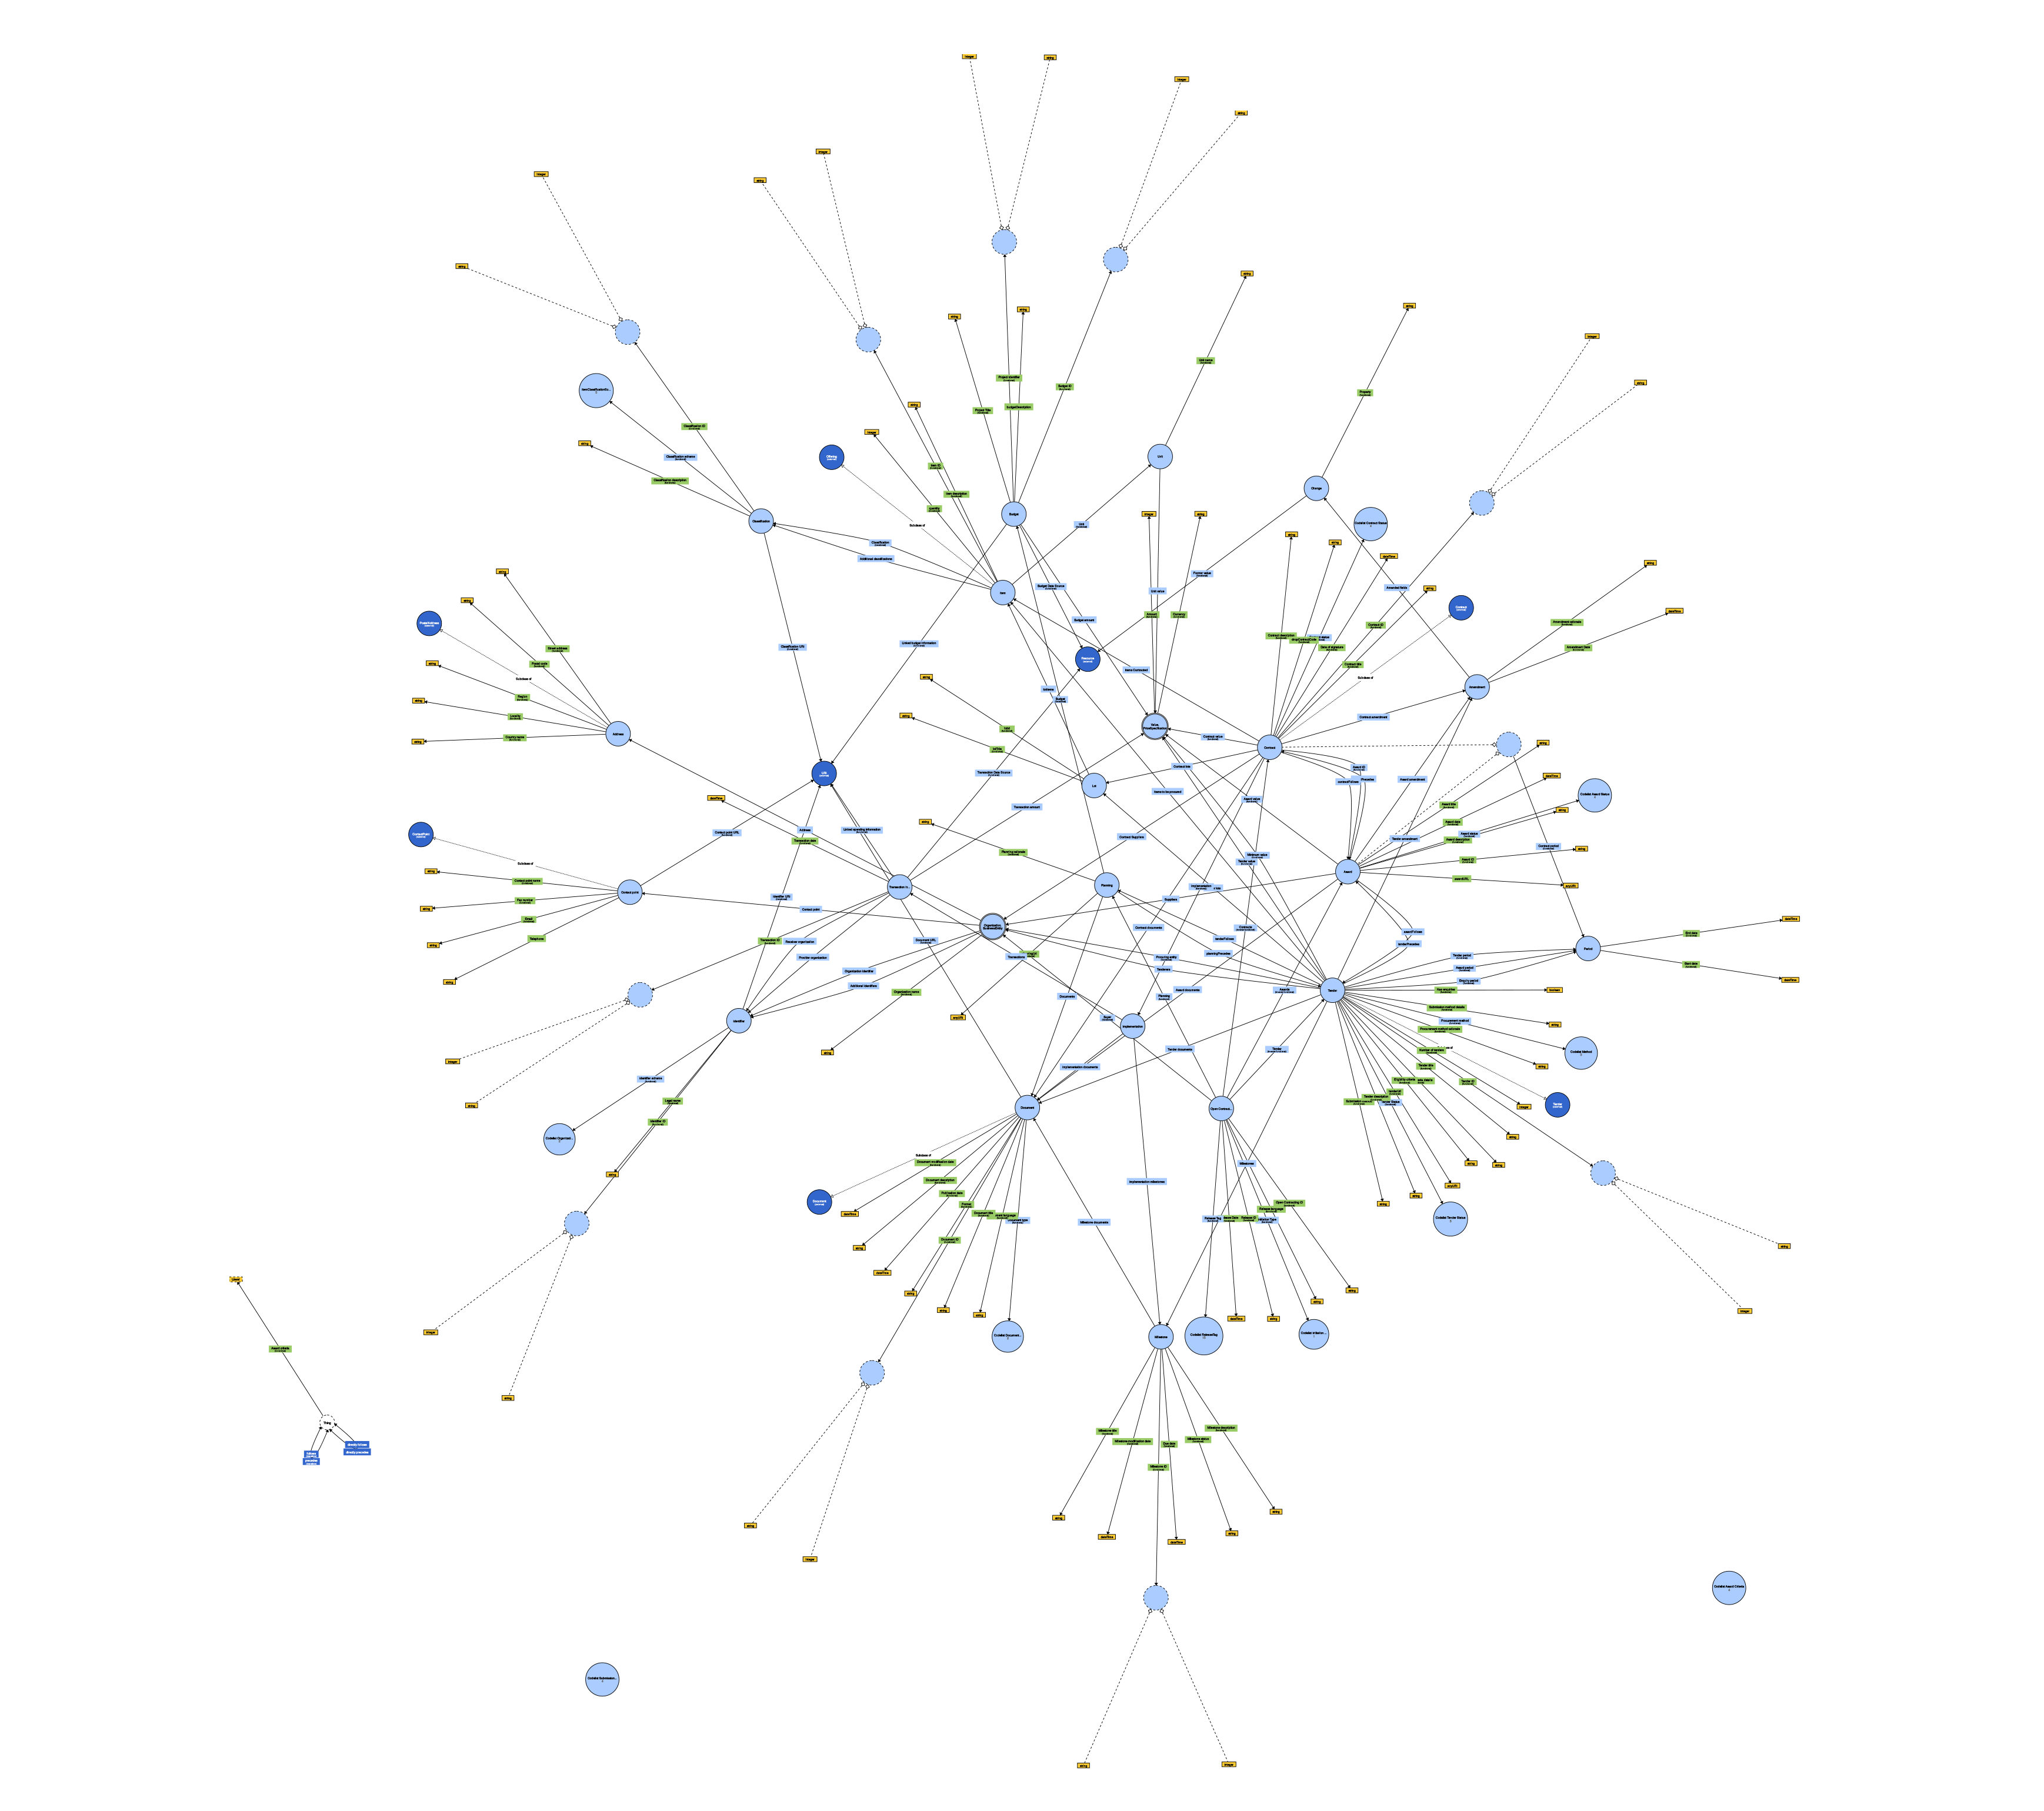
\includegraphics[width=180mm]{figuras/grafoOCDS.png}
    \caption{Grafo de la ontología desarrollada}
    \label{img:grafo ontologia desarrolla}
    \end{figure}